\chapter{第七期}

\section{2020年11月3日 星期二 晴}

夏天祺

“呜呜”,风娃娃不开心了,听起来像是沉郁的降B小调,开始呜咽了起来,这一呜咽,风更大了。满头金发的树木们纷纷用力的地摇着头。发出了“沙沙”的轻快的响声,正在坐公交车的我,早已把自己变成了一颗粽子。风娃娃这一呜咽,强烈的风呼呼地钻进了我的衣服里。我的脚就像一条倔强的活鱼一样,不停地扭动着。我生气地关上窗户,心中暗暗责怪这古怪的风。现在都已经深秋了,温度也变低了,人们都穿上了长衣长袖,大部分树木都换上了金色的树叶,星星点点的桂花散发着浓浓的香气,红色、白色、黄色的菊花纷纷地开了,橘子、柿子、柚子等各种水果都挂满了枝头,等着人们去摘呢!

\section{2020年11月4日 星期三 晴}

戴瑞彤

今天又是我最爱的无书面作业日,我早早地做完作业出去玩了。现在天气冷下来了,大家穿上外套,以便抵挡冷风的呼啸,大雁们飞向南方,寻找温暖的新家,树木们慢慢脱掉了身上厚重的金色外套,为大地铺上一块黄色的暖和的地毯,免得它着凉。不知不觉中,已经8:30了,也该回家了,我回到家,却发现闲言碎语还没写,唉,完蛋了,我只能赶紧补了。

\section{2020年11月4日 星期三 晴}

蒋鲁弋

今天中午,我们排队去吃饭,我已经闻到饭菜的香味了。

我像饿狼般向我的饭盒冲了过去,谁知一不小心撞到了另一份盒饭,那份盒饭掉在了地上,顿时汤汁乱溅,我身上全都是了。我呆呆地站在那里,不知所措,心想:完了完了,我闯祸了,衣服还脏了!怎么办啊!这时,老师又拿了一份盒饭,说:“吃完,清理一下”。我点点头,坐在另一个地方开始吃饭。

“心急吃不了热豆腐”,大家可不要像我一样哦!

\section{2020年11月4日 星期三 晴}

杨若君

今天晚饭过后,弟弟正在写一个句话。这时爸爸正好去倒垃圾了,妈妈走了过来说:“小宝你这个句号要改成逗号。”弟弟生气地道:“快走开!我明明是对的!”过了会儿爸爸回来了,他瞄了一眼弟弟的本子,也说:“小宝,这个改成逗号。”弟弟说:“好的,我上就改!爸爸你可真厉害呀!”我在一边小声说:“我的个妈呀!弟弟见到妈妈和爸爸简直不是一个人啊!”

\section{2020年11月5日 星期四 晴}

姜姸慧

今天老师叫了一些同学读昨天没读的周末五星作文,徐诚磊的《忘不了的餐厅有感》太精彩了。一开始,读到小老头小老太时,我们大家都笑了起来,可后来才知道那些老人们原来有老年痴呆。可当他读到如果我老了,你就把我送进养老院,我瞬间热泪盈眶,我根本无法想象妈妈没有了的世界,我的脑海里浮现了一些画面:走进厨房,那里空无一人,没有妈妈穿着围裙忙碌的身影;
走到阳台,也没了妈妈为我洗衣服的场景;走到梳妆台,妈妈为我梳着头发,可妈妈突然不见了,只留下那把木梳。我不争气的眼泪马上就要流下来了,可是硬生生的被我憋回去了。读完后,只见詹老师哭了起来。还说到:“这是你们每个人都会经历的。”我的眼泪终于忍不住流下来了。

\section{2020年11月5日 星期四 晴}

李卓涵

今天晚上,弟弟不知为什么一直在掏鼻子。老爸很生气,骂了弟弟,可还是不听。我提了个坏主意——把弟弟的手指上涂上芥末。老爸很生气:“要不也给你涂上?你不也咬手指吗?”我只好灰溜溜地走了。

\section{2020年11月9日 星期一 晴}

李朗

美术课时,我竟然忘带了马克笔!无助的我只能向徐诚磊借兵符——马克笔。徐诚磊拿着一支高光笔对我说:“你如果能说出这是什么笔,我的这桶马克笔就送你了!”哪有这样天降的好事!我立刻同意了,因为高光笔我见过,于是十分自信:“这是一支高光笔!”徐诚磊说不是,这是一支没水的笔。这时来欣年也加入了谈话,她说这是一支高光笔。被来欣年这么一说,徐诚磊立刻认了。我高兴地拿走了那一桶马克笔,还用修正带把上面“徐诚磊”的名字涂掉了,还写上自己的名字。不料,徐诚磊一把夺走马克笔,还说他不守信用。哼!徐诚磊真可恶!

\section{2020年11月11日 星期三 晴}

戴瑞彤

今天上午,我们迎来了数学期中考,本来我还想着晚点看到我那难看的成绩,可是现实是残酷的,拥有超快速度的章老师在下午就改完了我们的试卷。唉,面对现实吧。我想,章老师抱着一大叠改好的试卷走进了教室,对我们说:“这次我们班考得还不错,接下来让我报一下分数。”我的心一下悬到了嗓子眼儿,两只手的手心上不禁冒起了汗,紧张极了。“施迪文100,陈思涵98,戴瑞彤89……”章老师清楚地报着。“什么!89?!”我在心里暗暗想着。“那不是离90分就差一点点吗。”一盆无情的冷水泼在了我的脸上。

考试前不努力,考试后徒伤悲啊!

\section{2020年11月12日 晴 星期四}

姜姸慧

今天我们大家一起去江边毅行。来到江边,时有几丝微风吹过,有些凉意。江面上波光粼粼,但又很平静,和镜子一般。突然,一阵歌声打破了江面的宁静,也活跃了气氛。走着走着,就到了终点。这次毅行,让我学会了坚持,正如古话说的:“流血流汗不流泪,掉皮掉肉不掉队。”

\section{2020年11月16日 星期一 晴}

李朗

今天放学后,我和范思雯一起回家。走在路上,范思雯突然大叫:“有钱!”如果把我比作炸弹,“钱”无疑就是点燃我的导火索。我急忙低头一看,果然有一张5元面值的纸币。可能因为我是我们班足球队的吧,我的手速不快,“脚速”倒很快,一下子就踩中那张纸币。不过那张纸币最终的命运是被范思雯交给值周老师了,唉!

\section{2020年11月16日 星期一 晴}

杨若君

今天晚上弟弟正在读课文——小书包。这时弟弟说:“姐姐,你听我读一下改编版的小书包吧!”我同意了。于是他说:“我的小书包,啥宝也没有。就那一支铅笔,上课不安生,下课还乱跑。每天起得晚,害我总迟到。”我想:天啊!这把课文都改成啥了呀!

\section{2020年11月17日 星期二 阴}

夏天祺

昨天,我和李恩博、孙轩睿、姚琪等人都被学校的田径队选上了,看见同学们都用敬佩的眼光看着我的时候,我的心中非常开心,还夹杂一些骄傲。今天训练的时候我数了数,我们班的人足足有六个呢,是最多的,而且我们班的体育可是最强的,其他班肯定就是我们桌上的一盘菜,呵呵!在跑50米的时候,我的旁边站着一个大约比我高五六厘米的六年级学生,看起来跑步不算太快的样子。哨声一响,我就像一只猎豹一样冲了出去,可是旁边的六年级学生是一只比我更快的狮子,“嗖”的一声就冲到了我前面,后面的一个人也马上追了上来。到了后面的一段,我不断的给自己鼓劲,奥利给,终于跑进了前几名。现在我才发现我就是那只坐井观天的青蛙。总之,我以后一定要好好训练,争取以后的全区比赛可以选上我。

\section{2020年11月18日 星期三 晴}

戴瑞彤

天渐渐暗了下来,太阳就像一个光芒四射的大火球,照得我都睁不开眼睛,把世间万物都染成了金黄色。过了一会儿,太阳变得柔和了,颜色从金黄色变到了橘色,就像是一个巨大的橘子一样,正慢慢地往下掉。现在,太阳又变成了橘红色的,犹如一盏圆圆的红灯笼,也像一颗珍贵的红色大宝石,正发出着红色的美丽光芒,可爱极了!天边的云霞,远处的山,近处的房屋、树木,人都被笼罩在金红色的光芒之中。

原来生活中并不缺少美,只是缺少发现美的眼睛罢了。

\section{2020年11月18日 星期三 晴}

蒋鲁弋

星期一早上,我正在香甜的梦里,刚要吃到大汉堡的时候,老妈把我叫醒了。我看了一眼钟,才6点多!又躺了下去。老妈又把我从被窝里拉了出来。我不耐烦了,生气的说:“干嘛六点多就起床?”老妈说:“施同学生病不能上学了,老师教你顶替他当小红帽!”我一下子从朦胧睡意中醒来了,马上去了学校。

这可真是喜从天降啊!

\section{2020年11月19日 星期四 晴}

姜姸慧

这星期二吃鸡米花,可我不能吃,因为我要打蛔虫,不能吃肉。那鸡米花金灿灿的满是鳞片,看上去都很香,闻上去更…… 我吃饭都是憋着气的,要呼吸都是很快的。可到最后,我终于忍不住了,一口全放到了嘴里,真香!!!

\section{2020年11月19日 星期四 晴}

李卓涵

今天,我们去跳长绳。一直跳多没意思,我想。于是,我在跳的瞬间把小红帽戴上。施迪文嘲讽道:“耍帅!”我撇撇嘴,施迪文都养成习惯了,每次跳都会回一下头,这不算耍帅?接着,姚琪、孙轩睿和许智涵也开始学我。我都不玩了,他们还玩。我只好笑着指着自己说:“万恶之源!”他们也笑了。

\section{2020年11月23日 星期一}

付梦欣

今天放学前老师说,明天我们班和6班不仅要足球比赛,还要低碳博物馆参加讲座。老师没有讲完我就听到有人说“啊!这不会很累么?”老师好像听到了她说的话,又说:“我也没办法,校长说必须去,没有哪个班可以比得上5班和6班了。”这一刻,让我觉得既然校长信任我们班,我们班也要为校争光,更加努力。

\section{2020年11月23日 星期一 晴}

李朗

今天体育课下课时,我和宋旻峻哼起来黑人抬棺的旋律。哼着哼着,我突然灵机一动,用“妈”字代替“哼”,变成了“妈妈妈妈……”。宋旻峻听到我这样哼,也改成了“妈妈妈妈妈妈……”。听到宋旻峻也这样哼,我立刻改成了“奶奶奶奶……”,听到我这样哼,宋旻峻也换成了“奶奶奶奶……”,最后,竟变成了”姥姥姥姥……”!哼完之后,我俩都笑了。

\section{2020年11月24日 星期二 小雨}

李一阳

一下车,一阵微风吹过,他好像导游一样带着我和妈妈来到了花港观鱼。一条条五彩斑斓的小鱼在水中玩耍。水面上的荷叶不是墨绿的,不是浅绿的,也不是翠绿的,而是嫩绿的。一片片荷叶在水中摇晃,为花港观鱼增添了几分生气,也为小鱼找到了“避暑山庄”。

\section{2020年11月24日 星期二 雨}

夏天祺

上个周末,我和徐诚磊以及几个小朋友在小区的公园里玩捉迷藏游戏。这可不是普通的捉迷藏哦,这次的捉迷藏可以用手表通话,“鬼”和“逃生者”可以随处跑动,这次的活动范围也扩大了。一开始我和一些人躲在公园的桥底下,幸好我们都不算高,正好可以躲进去。我们屏息凝神,只听见我们紧张,急促的呼吸声。我的心呯呯直跳,就像一块大石头悬在了半空中。可是,当听见桥上的人走路时的“咚咚”的声音,我更加紧张了。突然,一股奇怪的笑意直冲我的嘴巴,我忍不住笑出了声,别人一看我笑,也跟着笑了起来。可是其中一个人笑得太大声了,暴露了位置,那个“鬼”却偏偏选择了我。那个小家伙跑的挺快,很快就追上了我,那悬着的石头上,好像又加上了一块更大的石头。过了一会儿,我已经累的气喘吁吁,那个小“鬼”好像一个机器人一样,一点都不累。我只好跑进树林里,钻进了一堆灌木丛里。那个“鬼”走了过来,我屏住呼吸,想着:我是空气,就当我不存在,他最终没发现我跑开了。裁判说,鬼一败涂地,逃生者大获全胜。

\section{2020年11月25日 星期三 雨}

戴瑞彤

这几天天气渐渐冷了下来,冬爷爷的脚步一点点逼近了。调皮的冷风娃娃一个劲儿地往我的衣服里钻,冻得我不禁颤抖了一下,连忙拉上了外套拉链。冷风娃娃还是不想就这么善罢甘休,依然在我的身边刮着,“呼——呼——”,我的耳朵受不了这寒风了,已经被冻僵了,进入了冬眠状态。我仿佛听到了这瑟瑟的寒风,正在得意忘形地笑着,我想:算了,随它去吧,跟这风有啥好计较的呢?

这风证明冬天来了,冬天已经来了……

\section{2020年11月25日 星期三 雨}

徐诚磊

今天放学以后,我迈着沉重的步子,向妈妈的车子走去。为什么?当然是因为学校里有很多作业未完成,要回家去完成,妈妈肯定要骂我一通。但上车,这种心情就被一扫而空,车上放了一堆书,要知道我可是好久没有新书看了呢,这可真是一场及时雨!想起我未完成的作业,不仅有一些愧疚,看来以后要在学校里天天向上,努力学习,不负父母期望!

\section{2020年11月25日 星期三 阴}

蒋鲁弋

今天体育课,老师说让我们踢足球。一开始还是很高兴的,后来因为我乌龙了一颗球,害我们输球了,心情就很郁闷。对方开始说我们“菜”,我们不服,说:“你们人多呀!10:16怎么打?”对方说:“你们是专业队呀,我们多几个人怎么了?”于是我们班所有的男生开始吵架,许同学还打人了,到了下一节课才平静下来。

哎,我技不如人,要是我没乌龙,人家也不会吵架了!我以后要好好练球,这样就不会输了!

\section{2020年11月26日 星期四 小雨}

姚琪

今天我一回到家,就被桌上那一盆绿意盎然的文竹吸住了眼球。它的叶子像松针一样,却又十分柔软,摸上去像摸鸭绒一样,它的茎和枝条差不多粗细。因此看上去像一根最顶端的树枝插在泥土里。那翠绿的茎和叶,配上漆黑的盆和棕黄色的底座,真是天衣无缝,妙笔生花啊!

\section{2020年11月27日 星期一 晴}

戴瑞彤

冬天的校园(一)

冬爷爷的脚步踏入了我们的校园,冬天在不知不觉中到来了。冬天的校园是多姿多彩的。我们学校里有一小片银杏树林,里面有几棵高大挺拔的银杏树,它们就像一个个强壮的士兵,时时刻刻都保护着我们的校园。如今,天气变冷,这些“士兵们”都脱下了绿色的长袖,换上了黄色的大衣,但渐渐的,黄色大衣也不暖和了,它们也脱掉了黄色大衣。可是这些大衣总不能浪费吧,银杏士兵们可有一副好心肠,它们把黄色大衣送给了大地,还热心地帮它盖上这条黄色大衣棉被,以防大地着凉。就这样,我的第一篇风景连载就拉开了序幕……

\section{2020年11月27号 星期五 阴}

徐诚磊

今天上“玩转科学”课时,我可真是度秒如年哪。可玩转科学不是挺有趣的吗?别急,请听我娓娓道来:我迈着快乐的脚步,走进教室,坐在位子上看老师今天又让我们做什么好玩的东西。“今天我们做桥梁模型。”老师宣布道。“万岁,模型最好玩了!”身边的拼装高手小琪说到。于是我迫切地打开老师发下来的盒子,刚打开盒子就被泼了一头凉水,里面竟然没有拼装方法。我只能自己弄,看旁边的同学都快把桥基座搭好了,而我只搭了一个方块,额头上冒出一颗颗黄豆般汗滴,唉,我真是度秒如年哪!

\section{2020年11月28日 星期二 晴}

夏天祺

今天是个特殊的日子,因为学校举行了一场足球赛。昨天和一班比赛我们是一败涂地,可今天我们要面对的是六班,要知道六班有两个魔鬼球员,一个是刘士一,一个是季子皓,他们都是校队的主力。我这次是后卫,是最后一道防线,所以这次的比赛压力都压在我和守门员王子彦的身上了。比赛开始了,六班先发球,只见刘士一就像一道闪电一样地把球踢了出去,只听见“啪”的一声,就传来了一阵欢呼声,原来六班直接进球了。我偷偷问了问王子彦,而他却什么都不知道,我终于见识到了六班的实力。过了一会儿,刘士一又带着球过来了,我心中的弦也紧绷着,接着他又把球传给了季子浩,我紧盯着球心怦怦直跳,他离我越来越近,我毫不犹豫地向他冲了过去,来了一个滑铲,我便闭上眼睛,任由上帝安排了,可当我睁开眼睛的一刹那,惊奇的发现我抢到了球,我急忙把球传给了前锋。之后,我又用滑铲断掉了六班好几个球,可是不知是对方的守门员太强,还是我们太弱,过了不久,六班就进了好多个球。此时,我怒火焚烧,刘士一又带球冲了过来,我感觉自己劳累的身体充满了力量,为了我们的班级,为了遵守我的诺言,我拼了!我用力地飞起一脚,球就像一颗子弹一样划破了天空,一下子从中场踢到了对方守门员的门前,六班的人都用惊奇的目光看着我。比赛结束了,虽然没有赢,可我遵守了我的诺言。

\section{2020年11月30日 星期一 晴}

我家的书架上有一盆文竹。它是我最喜欢的植物之一。文竹有着苍翠挺拔的树干,笔直笔直如同守卫在边疆的战士们,文竹的叶子是扁平的。有些文竹的前端是微卷的,像一个翘起来的“金色巴掌”;有些叶子边缘有些泛黄,给人一种渐变的感觉;还有些分叉口十分的明显,看起来玲珑可爱。整盆文竹与书架里的书融为一体,散发出一种书香之淡雅之气。真应得上这个“文”字啊!

\section{2020年12月1日 星期二 晴}

徐宸诚

今天打完羽毛球,肚子疼得咕咕叫。走回家时,看见旁边小店上有好几块饼,油亮亮的。我买了一块赶紧吃,说了也奇怪,我吃了一口肚子就不疼了!那感觉,真是飘飘欲仙啊!

\section{2020年12月1日 星期二 晴}

孙轩睿

踢完足球,回家已是四点多。但是应该不会走最最恐怖时候的“恐怖之路”,因为今天不坐公交车,坐同学妈妈的车回家。

不在最最恐怖时候的“恐怖之路”感觉一点儿也不恐怖。瞧,虽然路灯还没有亮,但是整体较亮。阳光散落在各处,营造出光明的环境,鸟儿们在一棵棵树之间唱着歌儿飞来飞去,像在嬉戏,又像在开联欢会,野猫不会突然从树丛里蹿出来,装神弄鬼地吓你一大跳,它们都趴在草坪边上,“喵喵”地叫个不停,好像在呼唤同伴来一起玩。四周一片和谐。

看来“恐怖之路”不是一直都恐怖的嘛。

\section{2020年12月2日 星期三 阴转小雨}

黄赫茗

今天是无作业日,放学后妈妈请我跟叶慕去餐厅吃饭,这是一个西餐厅,我们点了一个四人份的牛排套餐,套餐里面有一个牛尾汤,汤的颜色非常漂亮,但是放汤碗的盘子里还放了八角桂皮,我觉得我要被那个味道熏晕了,赶紧催妈妈快点喝完它,撤走!

\section{2020年12月3日 阴 星期四}

姜姸慧

近期,我们拉丁老师正在选春晚节目的人选,大家都努力极了!今天妈妈接到拉丁老师的电话,我心想:老师要干什么呢,突然打来电话。这时电话通了,妈妈接完后对我说:“你被老师选中春晚了。”我一听开心地一蹦三尺高。

\section{2020年12月3日 星期四 阴}

丁凝

昨天科学课时候,遇到难题,我习惯性的伸缩长橡皮,发出咯咯咯的声音,徐老师显然听见了,把眼光投向我,这是什么?我最喜欢这款橡皮了,都舍不得用,到底怎么啦?可没等我想完就有同学替我回答啦,这是橡皮,徐老师听了像是松了一口气,我还以为是裁纸刀呢,老师把橡皮当成禁用的裁纸刀啦,真是虚惊一场!

\section{2020年12月3日 星期四 晴}

李恩博

今天,我和同学一起玩。同学的衣服一不小心掉在地上,我赶忙上去拿起来,可是被同学看见,误认为“我”就是把他的衣服弄在地上的“大凶手”。他生气地从我的手中抢走了衣服,并打我了一下。我真的太冤了。我鼻子一酸流出来晶莹的泪水。我明明在帮助他呀!他却狗咬吕洞宾,不识好人心呀!即使我向前去为自己的清白而辩解,可是他非但不听,还来骂我。我就算跳进黄河也洗不清呀。我太难了!

\section{2020年12月3日 星期四 晴}

徐诚磊

今天准备睡觉时,电热毯开不了了。我试着自己搞弄了一会儿,电热毯依然开不起来。于是我便叫来了妈妈,说:“电热毯坏了。”妈妈便开始修起来了,只见她把电热毯的控温盒打了开来,用小刀、扳手等工具一顿修,电热毯就修好了,真是“万事通”老妈啊!

\section{2020年12月7日 星期一 晴}

付梦欣

我在前段时间内脚骨折了,打了石膏,所以上学就会比较难,需要爸爸妈妈一起送,爸爸负责背我,妈妈负责帮我拿书包。每次当我自己跳时,跳个一小会儿就累了,这时爸爸总会说:“算了还是我背你吧!”我点头同意,爸爸背上我没多久身体就有一点点发抖,看着爸爸头上的几根白头发心里暗暗发酸,想哭却怎么也哭不出来。

\section{2020年12月7日 星期一 晴}

余蕙琳

今天我又来到了银杏林,这是一个梦幻的地方。你能看到一只只“蝴蝶”翩翩飞落,为大地编织一块块鸭黄色的地毯,你能看见在树干上会有一只只神秘的叶蝶,你还能看见,雨过天晴,地面上的小水洼里,有一个小太阳,还有一朵朵小白云众星拱月般环绕着它,最重要的里面还有一片可爱的蓝天,蓝得如瓦蓝的大海般明亮。我爱小水洼,更爱银杏林。

\section{2020年12月7日 星期一 晴}

赵奕麟

最近我会跳长绳了,从一个甩绳的人变成了一个跳绳的人,只用了两天已经会连跳了。
第一天,我向我前面的李一阳请教一些小秘诀,李一阳说:“一开始,不要害怕,心里数到三就直接冲进去,不要跳。”经过几次训练后,我找到了感觉,就冲进去,跑到中心点一跳,然后快点跑掉,跳过几次后发现一次都没有成功,杨航熙说道:“要跑跳,等绳子到地就冲进去。”轮到我,我的心里默默数了三下,冲了进去,轻松一跃,我居然跳落过去了!果然只要成功一次,后面一定不会有很大的失败。

\section{2020年12月8日 星期二 阴}

余蕙琳

妈妈在我的书桌旁放了一盆小雏菊,它是那么清新、可爱,它的每一片花瓣都往外绽放盛开,这显得多么有生机。每一朵花的造型也不一样,最大的那一朵花曲直向上,朝着阳光那方生长。那4朵含苞待放的花苞努力地伸高脖子,想绽放明日的花朵。每一朵花都有自己的个性,像那朵半调谢半开着的雏菊,它知道自己的生命走向了尽头却仍不服输,努力睁眼去看清晨的朝霞。

\section{2020年12月8日 星期二 阴}

夏天祺

今天早上,一阵咚咚咚的声音吵醒了被窝里正在熟睡的我。只见爸爸急匆匆地跑进我的房间大声喊:“快醒醒,我们起晚了。”我漫不经心地看了看钟表,哎呀,我的老娘呀!真的起晚了。我急忙手脚并用地穿上衣服,一件、两件、三件,终于穿好了衣服,接着再是刷牙洗脸喝水吃饭,我和爸爸干完这些事情后,健步如飞的冲出了家门。可是今天非常奇怪,电梯过了一会儿就会进人,到了地下车库,我和爸爸赶紧上了车,可是连地下车库的门口都已经开始堵车了,还可以听见连续不断的喇叭声,喇叭声越来越急,我的心也越来越急。过了很久,我终于到达了学校,我一下车就飞快地朝学校奔去,似乎其它人进行的都是慢动作。最终,我“翻山越岭”又“爬山涉水”,终于在詹老师走进教室的那一刹那走进了教室。

\section{2020年12月8日 星期二 阴}

孙轩睿

以前,我认为送外卖很轻松,只要去餐厅拿一盒饭,送到客户家里就好了。但随着和外卖小哥的一次次接触,我开始改变想法,特别是昨天。

昨天我回来时,正在电梯里,正要关门,一个外卖小哥冲了进来。我暗暗打量他,他的皮肤黑黑的,眼睛流出露疲惫的眼神,头上挂着密密的汗水,乱乱的发丝从帽子里挂下来,显得十分劳累。再看看他的手机,屏幕都碎了,边边角角都已经破了,看样子这个手机他用了很久都没换过了。

“叮”电梯门开了,外卖小哥快步走出电梯,而我还在里面出神。

\section{2020年12月9日 星期三 阴}

许智涵

今天我要去做马赛克,刚到教室孙轩睿和沈冠屹过来和我说:“许,今天放学你等我一下”。“OK,要不你跟我一起回去吧!反正近。”“那就好办了,沈冠屹也来哦!”好嘞!就这样,这个事情埋下了引子…… 放学了,我在校门口等孙轩睿和沈冠屹,可等了十几分钟他们也没来,就在我以为他们俩已经回去时,三个人一边说笑一边吃东西走了过来,“咦?杨航熙也来了,”孙轩睿说,“嗯,老杨跟我们一起!”说着,二人便上了车,开到了拐弯处,爸爸还想再带上杨航熙,可杨航熙突然冒出了一句:“我妈说,别人的车子不能随便坐!”坐在一旁的孙轩睿大喊道:“这车上都俩人了,你还怕个啥!”

今日汽车载客:5人

\section{2020年12月9日 星期三 阴}

戴瑞彤

冬天的校园(二)

已经过了大雪,其它的花基本都抵挡不住那刺骨的寒风,纷纷凋谢了,而就在我们学校里一个不引人注目的地方,几棵山茶树上开出了一些深粉色的花。它们争相开放着,有的山茶花含苞待放,就像一个害羞的小姑娘,不敢探出头来看看这美丽的世界;有的山茶花只开了一半儿,如同一个正在熟睡的孩子,被人叫了起来,还恍恍惚惚的,处于睁一只眼闭一只眼的状态;还有的山茶花完全开放了,犹如一位美丽大方的少女,正向大家展现着自己呢!远远看去,这不就是“万绿丛中一点红”吗?连如此不引入注目的地方都有如此妙不可言的景象,看来生活中并不缺少美,只是缺少发现美得眼睛罢了。

\section{2020年12月10日 星期四 阴}

丁凝

正在上兴趣班,忽然一群人围在升旗台一角,我挤进去一看是一只小鸟,小鸟左翅出了很多血,上面羽毛凌乱,正缩成一团,眼睛疑惑地盯着我们。我轻轻捧起她,按照老师的指示,小心的把它放到围墙外。他回头看了两眼,毅然朝马路对面跑去。一辆车,两辆车,三辆车快要过了,我的心提到了嗓子眼。有一辆车,从到后面经过,但轮子一歪直接撵了上去后。过后,他被压死了,一个鲜活的生命,就这样消失了,可我的手上还残留他的余温,但这余温属于的生命已经消失了,在前一秒,我深深地体会到了世界的残酷和生命的脆弱。

\section{2020年12月14日 星期一 阴}

陈思涵

昨天晚上,我醒了。看到窗帘后面隐隐约约的有一丝丝微微星光,便准备去看看时间。可是,我突然有些害怕了,我想起看过的那些什么关于鬼啊,有幽灵飘动的“快讯”,心头不由得一颤,我发觉我背后冒出了一点点冷汗。我的手伸出被窝准备拿小夜灯,又快速缩了回来。我鼓起勇气,拿到小夜灯,打开并快速穿上鞋子,看了时间。

\section{2020年12月14日 星期一 阴}

叶雨飞

明天,有一场重要的活动,体育节个人项目比赛!我将代表我们班去参加一分钟双飞的比赛。双飞可是我无人能比的项目,这次,我下定决心一定要拿到冠军!我的最高纪录是127个,最多连续跳过183个!别说五年级了,就是全校女生,我也一定是名列前茅!我班男生都没我跳的多,都没我跳的快,只有羽毛球校队的人和我一般水平。当然,想拿到好成绩,也是要练习的。不多说了,我该去跳双飞了!

\section{2020年12月14日 星期一 阴}

黄雅嫣

今天上美术课时,我看了看自己的马克笔,又看了看后面那位富豪的马克笔,真的是应了那句话:没有对比就没有伤害。我转过身来,对许智涵说,“能借我一支灰色马克笔吗?”许智涵大方地同意了,我选呀选,选中了一只灰蓝色的马克笔。可一往纸上一画,唉,怎么画出来是紫色,我一问许智涵,他马上说这支笔确实是这个颜色,原来富豪的马克笔颜色有问题。

\section{2020年12月14日 星期二 晴}

赵奕麟

星期日,正在读英语,要发语音到微信群中,突然蔡老师发了一条语音:这里的“some”读错了。我订正完后,又发了一条正确的语音到群里,蔡老师又发了一条消息:恭喜第五单元考了100分!我一下僵住了,不知是高兴还是伤心,我半信半疑,怀着疑问的状态问蔡老师,消息发出时,我心中小鹿乱撞。蔡老师秒回:100微笑。我惊讶了半天。调整好心情后,又和蔡老师唠了一会儿嗑。原来师生之间可以那么快乐!

\section{2020年12月15日 星期二 晴}

徐宸诚

我开始写作业了,先拿出写字本,准备开始写。我突然害怕地想到:我是不是拿错写字本了!如果拿错了,我就要被爸爸妈妈死死地盯着,被老师责怪。唉,一切就只能听天由命了!于是我就把它翻到二十三课的最后一页,紧紧地按住纸角慢慢地往后,我手心的汗都出来了!耶,是26课!这一瞬间,我高兴得一跳三尺高,所有的烦恼都被我丢在了脑后。这一刻,家就是欢乐的海洋!但马上迎来的却是手臂的酸痛。

\section{2020年12月15日 星期二 晴}

孙轩睿

体训队训练完,我累得半死,姚老师说体育办公室有牛奶,每个人可以去办公室里排队拿一杯。当时我认为办公室的牛奶充足,每人都能拿到。可是发生了变故。

来到台阶前一个先进去的人走出来,向后面的宣布:“只剩下三杯牛奶了!先到先得!”我一听,天哪,只剩三杯了,看来我要抓紧了。这时,我余光扫到后面有几个人书包都没背就跑来了。我的天,如果他们一到,我肯定没得喝了。在“必须拿到牛奶”的信念的鼓舞下,我一个冲刺,三个台阶三个台阶一步走,再冲刺,一头撞进了办公室。拿起牛奶,我迫不及待地打开,喝一口,哇!浓浓地奶味在嘴里散开,真是太好喝了。

看来只要有目标或者信念,就一定能成功。

\section{2020年12月15日 星期二 晴}

杨航熙

《四季之美》曰:“冬天是最美的早晨”。

今早望天于东,见云色深,围似镶金。光于云隙透出,犹如金色利剑,直刺大地。吾见阳于东而升,阳先如咸蛋黄,令人垂涎。后如金色火球腾空,而云似车。见此景,故吾曰:“此景不如神话,何如神乎?”

故曾有人云:春之景,不及冬之晨。

\section{2020年12月16日 星期三 晴}

许亦凡

今天下午,要进行交接棒比赛,我们班每年田径都是第一,今天肯定又是第一名。想着想着,老师便叫田径队员到操场上去准备,不是田径的我们只能在教室里看书,可我们“身在曹营心在汉”,一直不停地默默地在为我们田径队助力。后来,成绩下来了,是第二名。没夺第一名的我们会越战越勇。明年勇得第一。

\section{2020年12月16日 星期三 晴}

戴瑞彤

冬天的校园(三)

寒冬降临,冬天的早晨,满天雾气腾腾,十步不见人影,大杨树上乌鸦不叫了,太阳盖着厚厚的棉在睡觉,小朋友们也穿上了厚厚的羽绒服。饭后,在校园中漫步,天气还是阴沉沉的,空气布满了厚厚的,低低的、灰黄色的浊云,给人一种压抑感。东北风呜呜地吼叫着,肆虐地在校园里奔跑,它仿佛握着一把锐利的刀剑,能刺穿严严实实的冬装,更别说那暴露在外面的皮肤,被它划了一刀又一刀,疼痛难熬。不久,我的脚也被冻僵了,大地简直变成了一块冷冰冰的钢板,把我的脚冻得生疼。

还是赶紧回教室暖和一下吧。

\section{2020年12月16日 星期三 晴}

施迪文

今天,我们五年级进行了跑圈比赛。由于我们前几次都是第一,因此这次我们信心满满。刚开始,我们遥遥领先。渐渐的,我们麻痹大意了起来。没想到,四班趁我们不注意,超过了我们…… 我们得了第二名。

从中,我悟出了一个道理:在取得成就后,不能骄傲,否则就会被别人超越。

\section{2020年12月17日 晴 星期四}

姜姸慧

前几天老师正在上课,那天上的课文是古人谈读书,正当我们在读:默而识之,学而不厌,诲人不倦时,只见宋旻骏一本正经的对王子彦说:“诲人不倦,汇仁肾宝片,他好,家才好。”这把在认真读课文的我笑喷了!

\section{2020年12月17日 星期四 晴}

余蕙琳

我越来越喜欢书桌上这个小小的台灯了,它给我带来光明与温暖。在我阅读时它带来了光明,它把光照在书上,而我的眼睛里也有了那个小小的影子。在寒冷的冬天,我发红的小手摸摸台灯微热的灯炮,瞬间暖流涌入心中,这是它给我带来的温暖。在我们身边,有许多微不足道的东西,但它却是那么有用。

\section{2020年12月17日 星期四 晴}

李卓涵

今天,詹老师教我们做了一个游戏——绳子上放一个乒乓球,然后将球传递给下一根绳子。说起来简单做起来难。好几次我们都在传递时出了问题。孙轩睿想出了一个“办法”,每当我们传递时,孙轩睿就抓住球将它放在下一根绳子上,然后立马就成功了。孙轩睿大喊“成功啦!”
,我们也跟着喊。

…… 真会掩耳盗铃。

\section{2020年12月17日 周四 晴}

姚琪

下午,老师带着我们做了一个小游戏——接绳。我们八个女生将四根强子围成“井”字形,并拉直。话不多说,由一个女生将乒乓球放在第一根绳子上,随着球慢慢移动,我们的心弦也渐渐拉紧。到我这根啦!我集中注意力,小心翼翼地挑着绳子,碰到第三根绳子了,我移动脚步,将球轻轻向下放,成功了!“耶!”一声,我们顺利地将球经过“最长”路段来到了终点。看来,团结往往能创造出美好的境界!

\section{2020年12月21日 星期一 晴}

赵奕麟

近日,哥生病。昨晚哥起倒水,洗鼻,出声,让妈听之,妈亦起,给哥药,无用,测温,则发现哥热也。早,爸带哥去医,验血,后发现哥淋1少,致急2,后之在家休。妈把家一分为二,一隔3,另一为安4,防哥传5我。

注释:1淋巴细胞百分比。2急性上呼吸道感染。3隔离区。4安全区。5传染。

\section{2020年12月21日 星期一 晴}

叶雨飞

跑50米乘8,班里绝对没人超得过我。我的成绩一直在男生优秀水平上徘徊,全年级也是数一数二的。今天,男生跑得最快的人也要1分35秒,我只用了1分32秒,毫无悬念又是第一。但是,我50X8最快能达到1分29秒,而400米最快可以达到1分26.89秒。所以,我一定要超越自我,刻苦练习,让50米乘8跟400米一样快,突破极限!

\section{2020年12月21日 星期一 晴}

余蕙琳

今天学校给大家发了一只时间管理器。我收到的是一只小猪圆形的管理器,这只小猪十分可爱,圆圆的身子,肉嘟嘟的脸蛋,两只大如玛瑙的黑眼睛,还有一个十分有特色的大鼻子。悄悄告诉你,我现在正用这只粉红小猪管理器计时我的闲言碎语写作时间呢!

\section{2020年12月21日 周一 晴}

王子彦

今天中午,孙轩睿、赵奕麟、孔俞澄几个人和我一起玩一个被他们称做“斗尺子”的游戏,就是用自己的尺子把别人的尺子撞下桌子。正玩着,詹老师推门走进来,看到我们正拿尺子撞来撞去,便严厉地问:“你们在干什么?”我们都被吓住了,我小心翼翼地回答:“在玩尺子。”“尺子是用来玩的吗?”詹老师上前一步,继续问。也不知谁用很小的声音讲了两个字:“不是……”詹老师再次说:“那你们还玩!”我们都不作声了,各自回到了各自的座位上。到了下午,我们几个又一次玩起了“斗尺子”,又不知道谁把尺子弹飞了出去,砸中蒋欣恬的玻璃水杯,砸出了一个破洞,水洒一地。詹老师知道后,十分生气,把我们批评了一顿,让我们清理干净地面,跟蒋欣恬道歉,赔她一个新杯子。詹老师也告诉大家,课间不要玩危险游戏,以及不要带玻璃水杯。

\section{2020年12月22日 星期二 晴}

夏天祺

一场残酷的战斗终于结束了,急性肠炎终于被我打败,我又可以重返学校了。放学后,我坐着公交车到了小区,一到小区门口,就看见几个送外卖的人,匆匆忙忙地拎着一大袋东西跑来跑去,我想他们一定是为了让自己过上幸福的生活而奋斗吧。还可以看见两三个环卫工人拿着扫把扫着地上的落叶,或者修剪着旁边的花草。我走过一座桥,就可以看见一个大公园,有许多小孩在嬉戏欢笑着,也有许多老人正在悠闲地聊着天,构成了一幅和谐的小区风景图。

\section{2020年12月22日 星期二 晴}

徐宸诚

今天早上,一到学校,一位同学就拉着我,带我到了卫生角,让我拿下口罩细细地闻这儿的“香味”。于是我就拿下口罩,嗅了嗅,真是不闻不知道,一闻吓一跳!那味道真是太浓了,我都不知道应该用什么词语来形容了!又过了一会,詹老师来了,听到我们在说这件事,于是就拿来了一瓶花露水,喷了两下,卫生角终于好了,发出了诱人的香味。董迈闻到了这一股香味,就说:“啊!真香!”

\section{2020年12月23日 星期三 晴}

黄赫茗

突然意识到自已已经五年级了,再有一年就要跟老师还有一些同学分开了。时间过得真快,记得一年级刚开学那会,我因为找不到座位而绕整个教室好几圈,最后只好随便找了一个座位坐下,现在虽然换了无数次座位,我再也不会坐错。唉,时间,如果人生若只如初见,那该有多好啊!

\section{2020年12月24日 周四 晴}

姚琪

今天下午阳光体育时,我们在多人跳长绳。一轮接一轮,我刚得了“冠军”在旁边休息。“哈哈哈……”一串清脆悦耳的笑声响起,原来是王子彦在跳时,不知道什么原因,他右脚踩在了左脚上,整个人飞了出去,并“完美”降落——摔在了地上。我的天啊!虽然这件事情很搞笑,但也很危险,大家千万不要模仿哦!

\begin{figure}[htb]
    \centering
    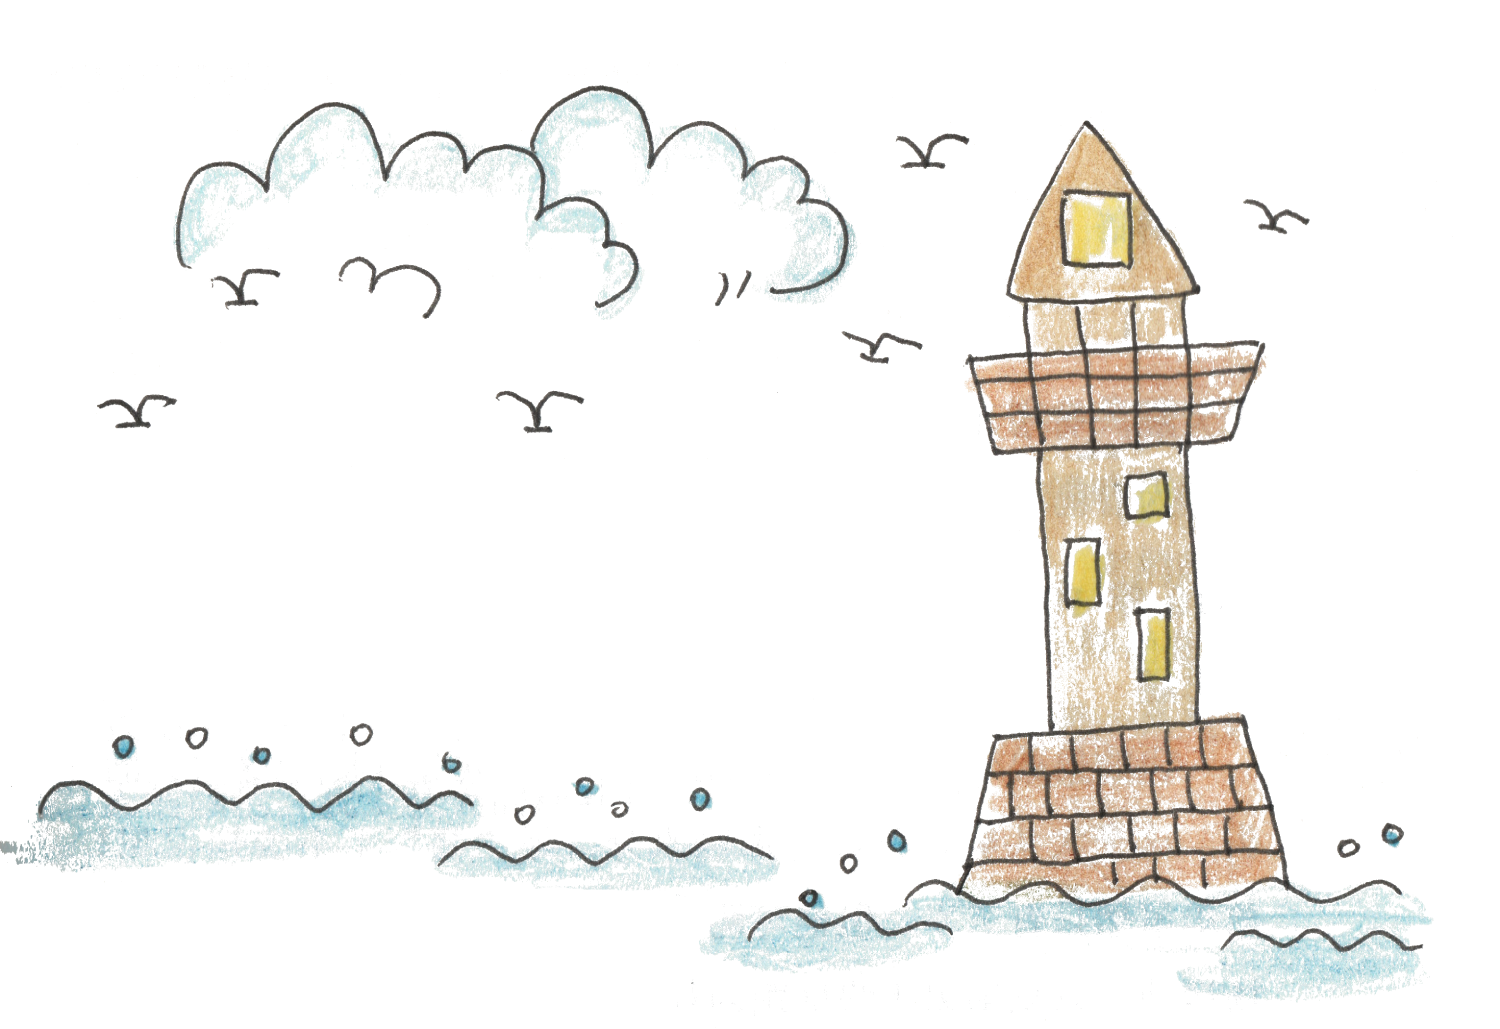
\includegraphics[width=\textwidth]{figure/07.png}
\end{figure}